\chapter{Análisis de Resultados}

La construccion de la antena finalizo con todas las partes mecanicas y electronicas ensambladas. A continuacion se presentan los resultados obtenidos en la caracterizacion de la antena.\\

\begin{figure}
    \centering
    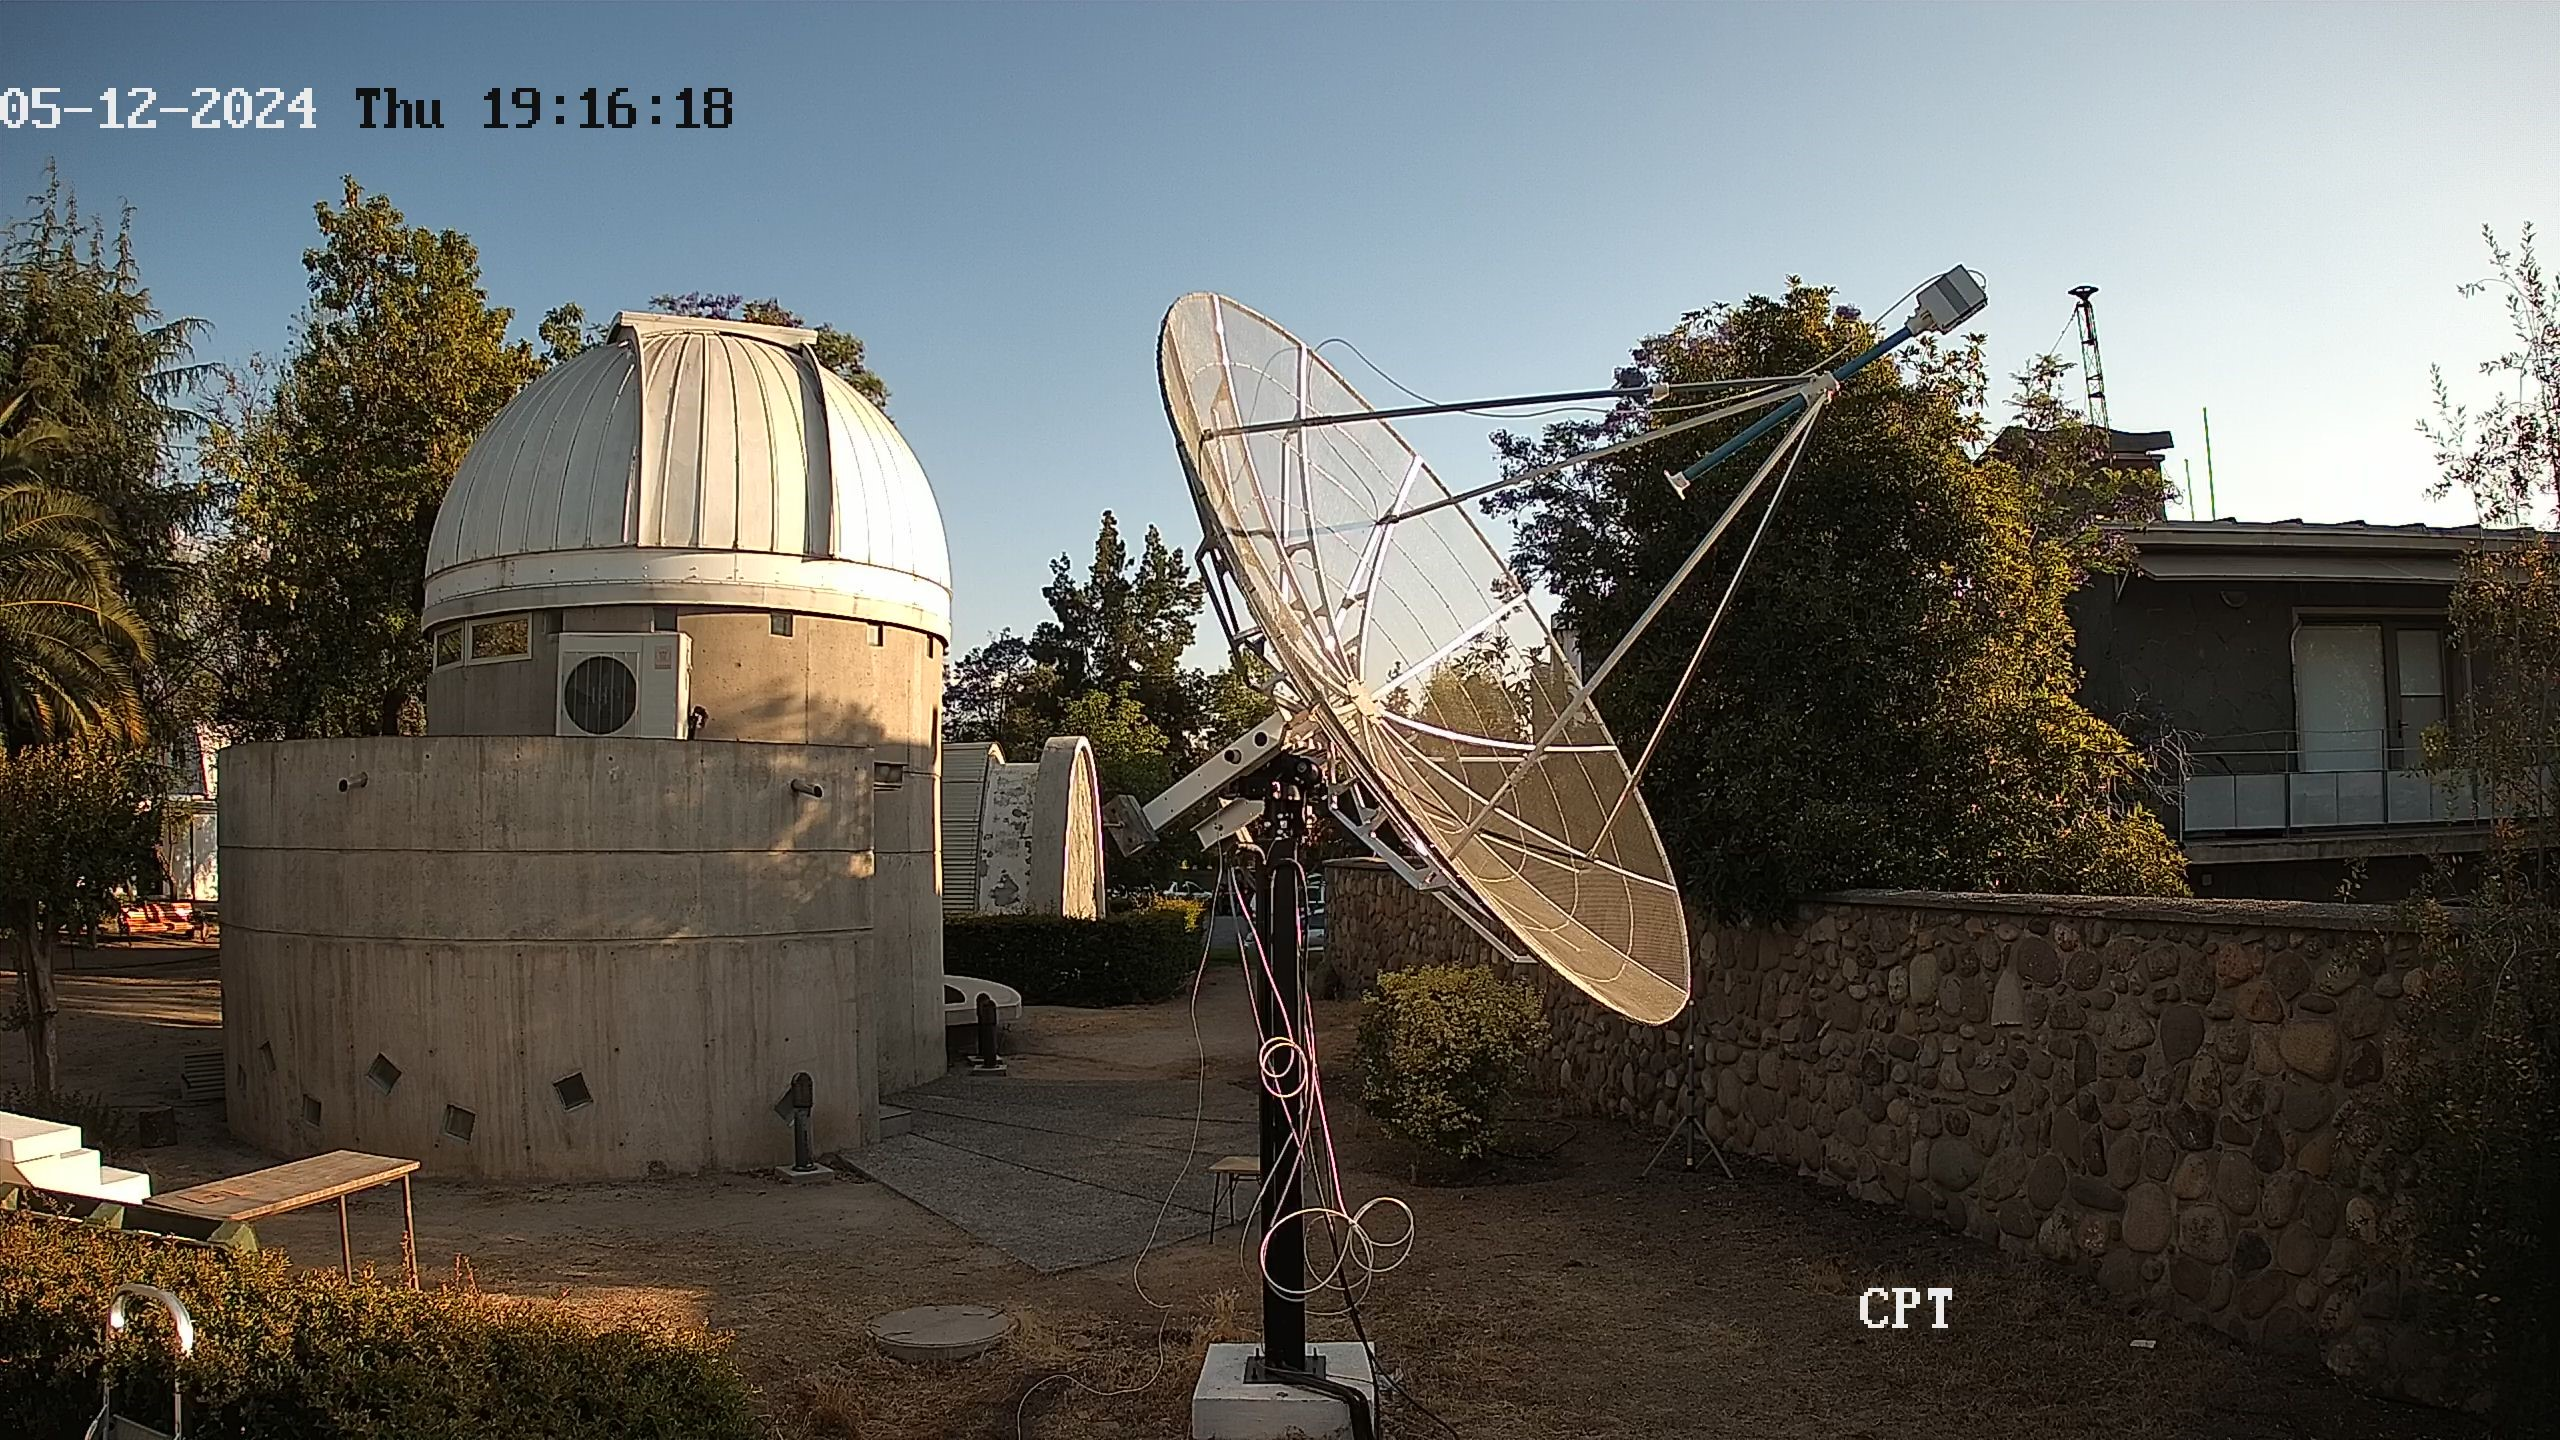
\includegraphics[width=0.8\textwidth]{img/antenna}
    \caption{Antena construida siendo monitoreada por la camara remota}
    \label{fig:antena}
\end{figure}

\section{Posicion del alimentador}

La posicion del alimentador con mayor ganancia se obtuvo a 135 cm de la superficie del reflector. La figura \ref{fig:distancia} muestra la ganancia en funcion de la distancia del alimentador al reflector.\\

\begin{figure}
    \centering
    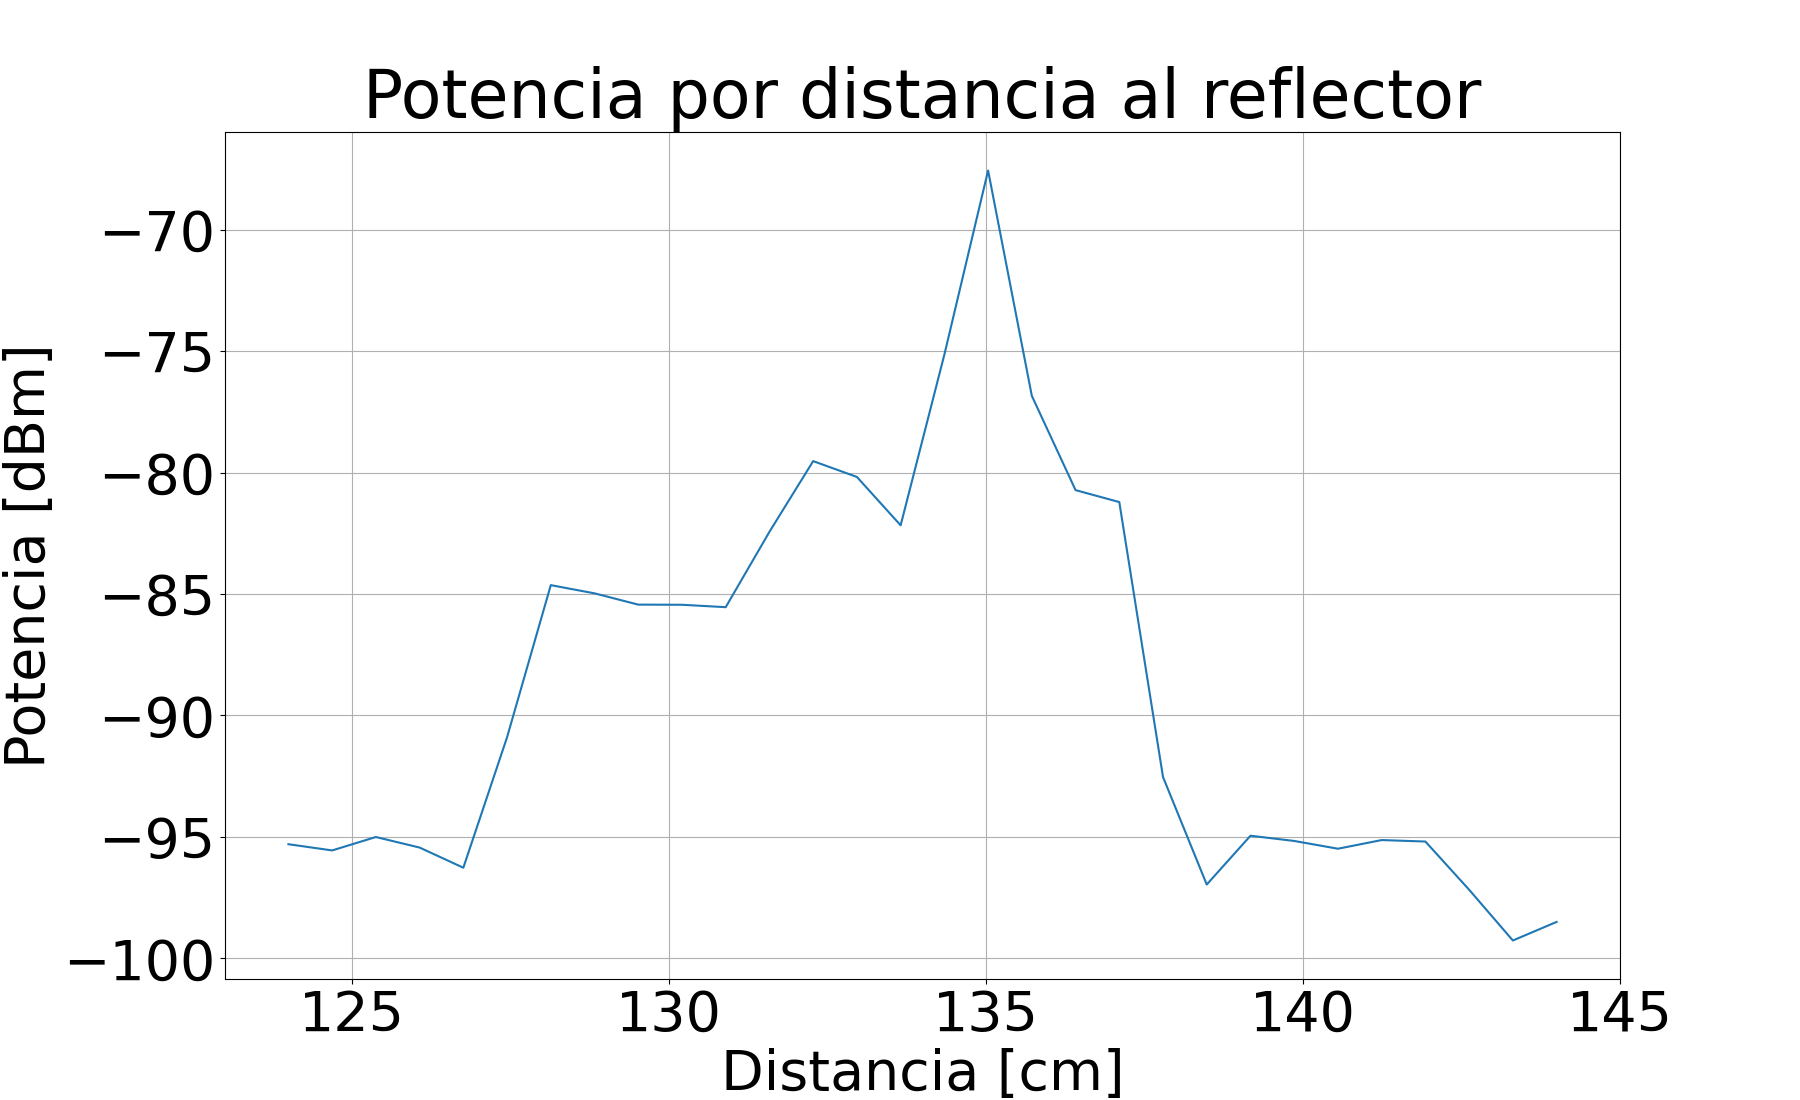
\includegraphics[width=0.8\textwidth]{img/enfoqueDist}
    \caption{Potencia recibida en función de la distancia del alimentador al reflector}
    \label{fig:distancia}
\end{figure}

La distancia obtenida coincide con la disatncia focal de la antena y se observa que la a medida que el alimentador se aleja del foco, aumentando o disminullendo la distancia con la parabola, la ganancia disminulle drasticamente perdiendo 6 dB por centimetro hasta llegar a la ganancia que tendria la antena sin considerar el reflector.\\

Estas perdidas son analogas a la medida de 1420 MHz para la de 400 MHz.\\

\section{Patrón de radiación} \label{sec:patron}

A continuacion se presentan los patrones de radiacion obtenidos para la antena a 1428 MHz y 400 MHz. Para la banda de 1428 MHz se realizaron los 2 cortes de elevacion y azimut ya que este se obtuvo utilizando el digitalizador del receptor, lo que permite hacer las maniobras de elevacion completas. En cambio para 400 MHz, se debia utilizar un cable coaxial hacia el analizador de espectro.\\

% \begin{figure}
%     \centering
%     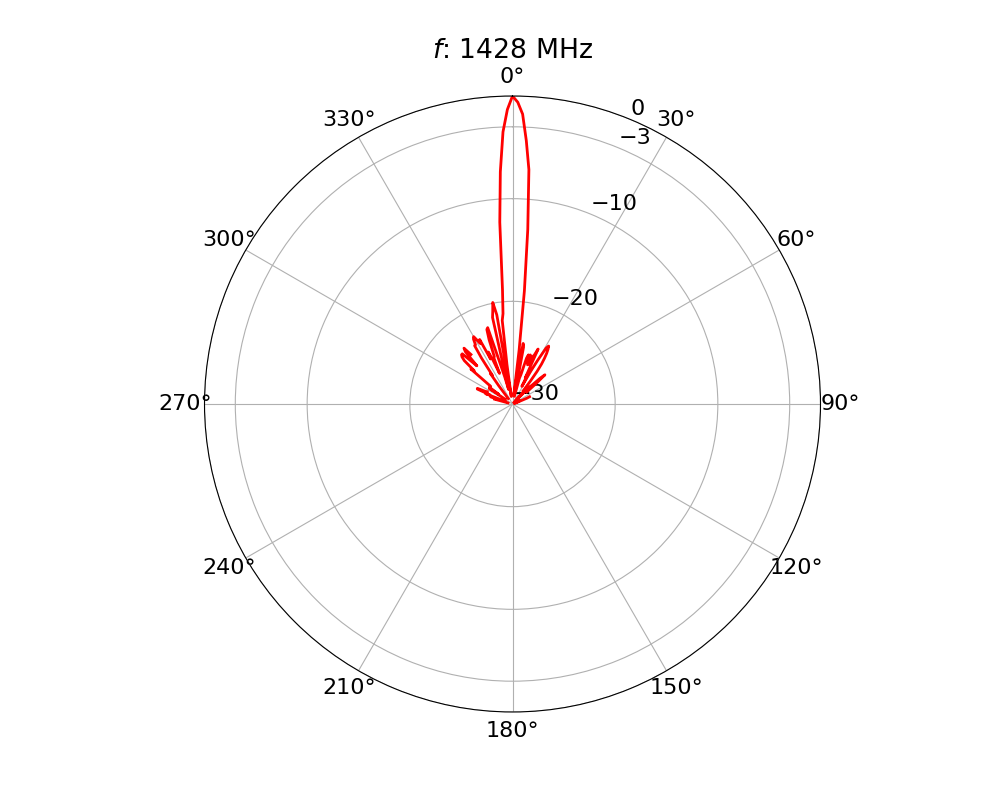
\includegraphics[width=0.8\textwidth]{img/1420rp}
%     \caption{Corte azimutal patrón de radiación a 1428 MHz}
%     \label{fig:1420rp}
% \end{figure}

% \begin{figure}
%     \centering
%     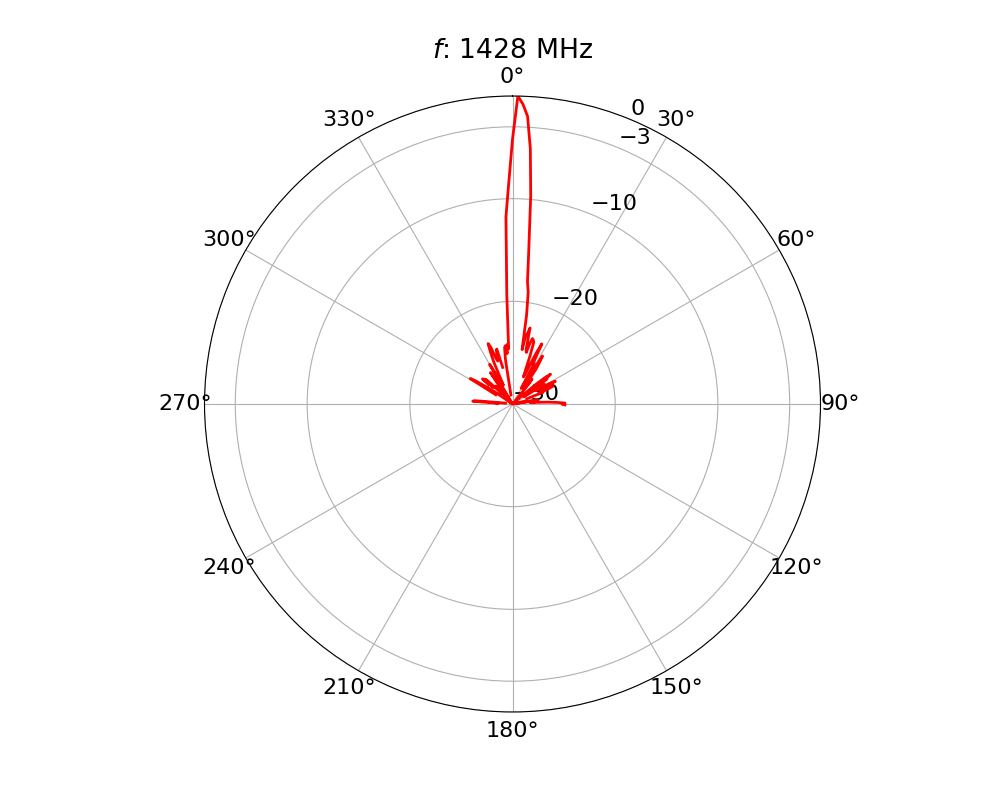
\includegraphics[width=0.8\textwidth]{img/1420rpel}
%     \caption{Corte elevacion patrón de radiación a 1428 MHz}
%     \label{fig:1420rpel}
% \end{figure}



\begin{figure}
    \centering
    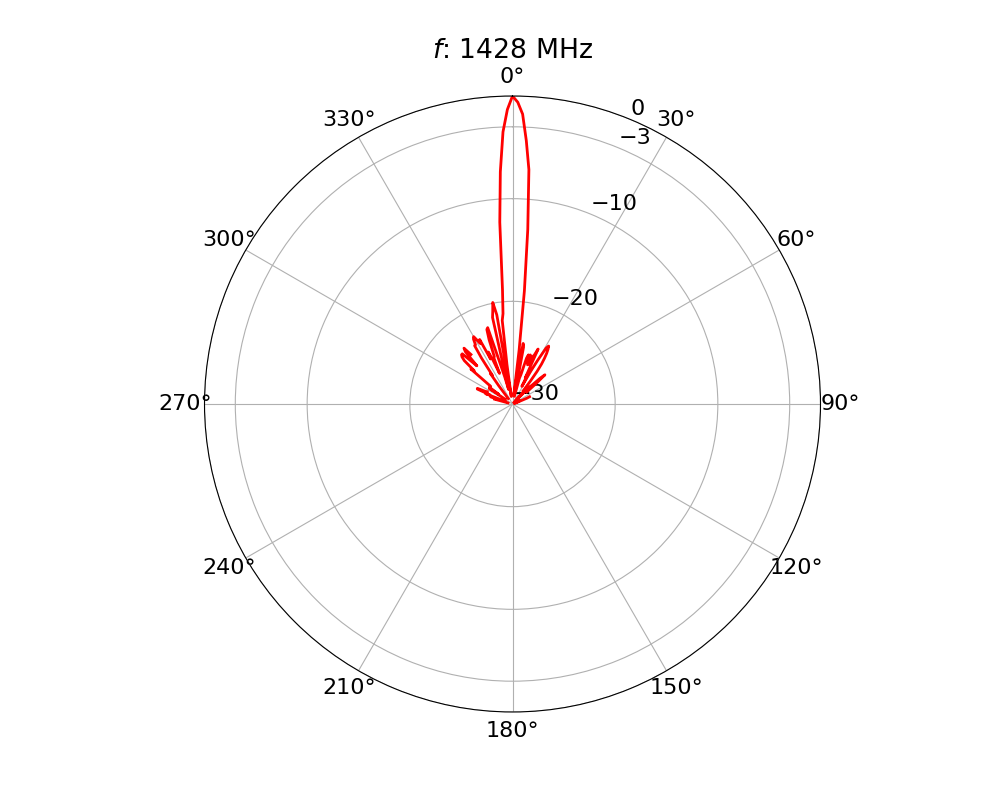
\includegraphics[width=0.8\textwidth]{img/1420rp}
    \caption{Corte azimutal patrón de radiación a 1428 MHz}
    \label{fig:1420rp}
\end{figure}

En la figura \ref{fig:1420rp} se observa el corte azimutal del patrón de radiación a 1428 MHz, donde se aprecia un lobulo principal predominante de 4.4 grados de HPBW y todos los demas lobulos laterales bajo -20 dB.\\

\begin{figure}
    \centering
    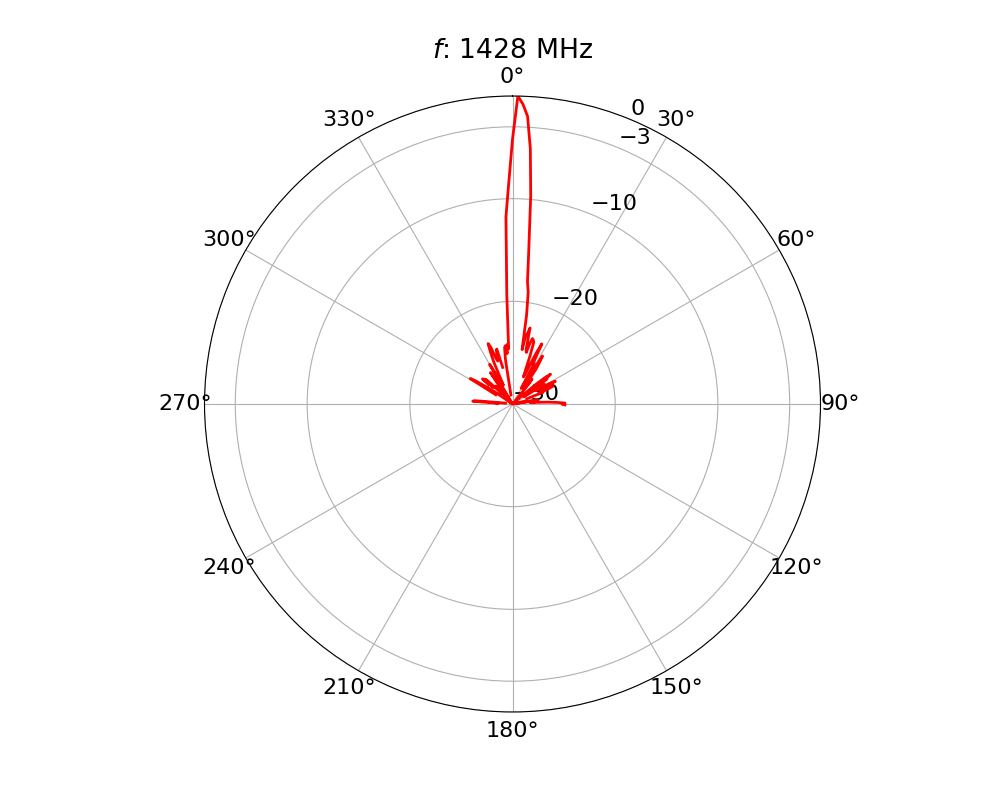
\includegraphics[width=0.8\textwidth]{img/1420rpel}
    \caption{Corte elevacion patrón de radiación a 1428 MHz}
    \label{fig:1420rpel}
\end{figure}

Con respecto al corte de elevacion, de la figura \ref{fig:1420rpel}, se observa un lobulo principal de 4.3 grados de HPBW y una discontinuidad en el lobulo principal a 0 grados. Los lobulos laterales  se encuentran por debajo de -25 dB.\\

\begin{figure}
    \centering
    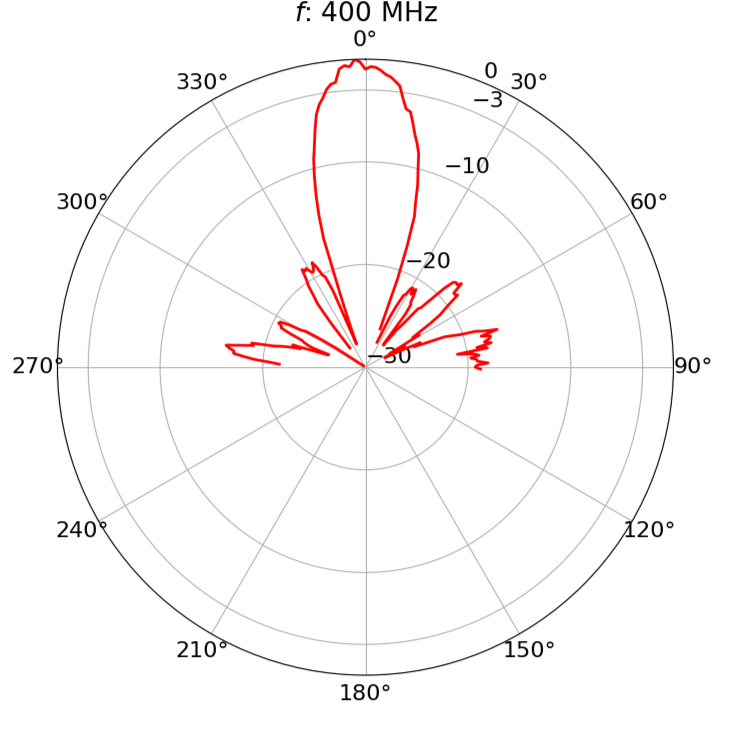
\includegraphics[width=0.8\textwidth]{img/400rp}
    \caption{Corte azimutal patrón de radiación a 400 MHz}
    \label{fig:400rp}
\end{figure}

En la figura \ref{fig:400rp} se observa el corte azimutal del patrón de radiación a 400 MHz, donde se aprecia un lobulo principal predominante de 7.5 grados de HPBW y todos los demas lobulos laterales bajo -15 dB.\\

\begin{figure}
    \centering
    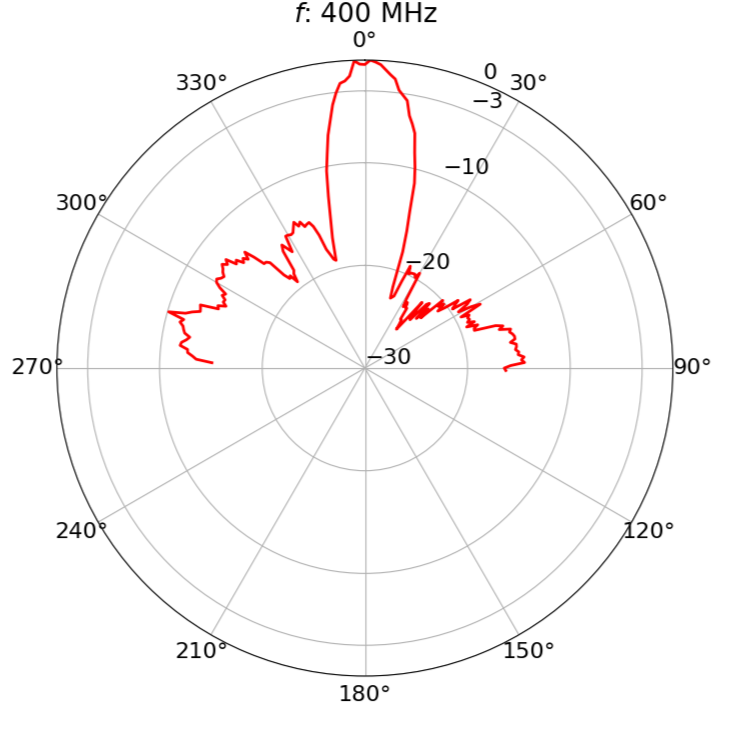
\includegraphics[width=0.8\textwidth]{img/400rpel}
    \caption{Corte elevación patrón de radiación a 400 MHz}
    \label{fig:400rpel}
\end{figure}

Con respecto al corte de elevacion, de la figura \ref{fig:400rpel}, se observa un lobulo principal de 7.5 grados de HPBW y una discontinuidad en el lobulo principal a 0 grados. A diferencia de la figura \ref{fig:400rp} los lobulos laterales estan dominados por ruido, sin embargo, sigue por debajo de los -15 dB\\



\section{Sensibilidad}

\begin{figure}
    \centering
    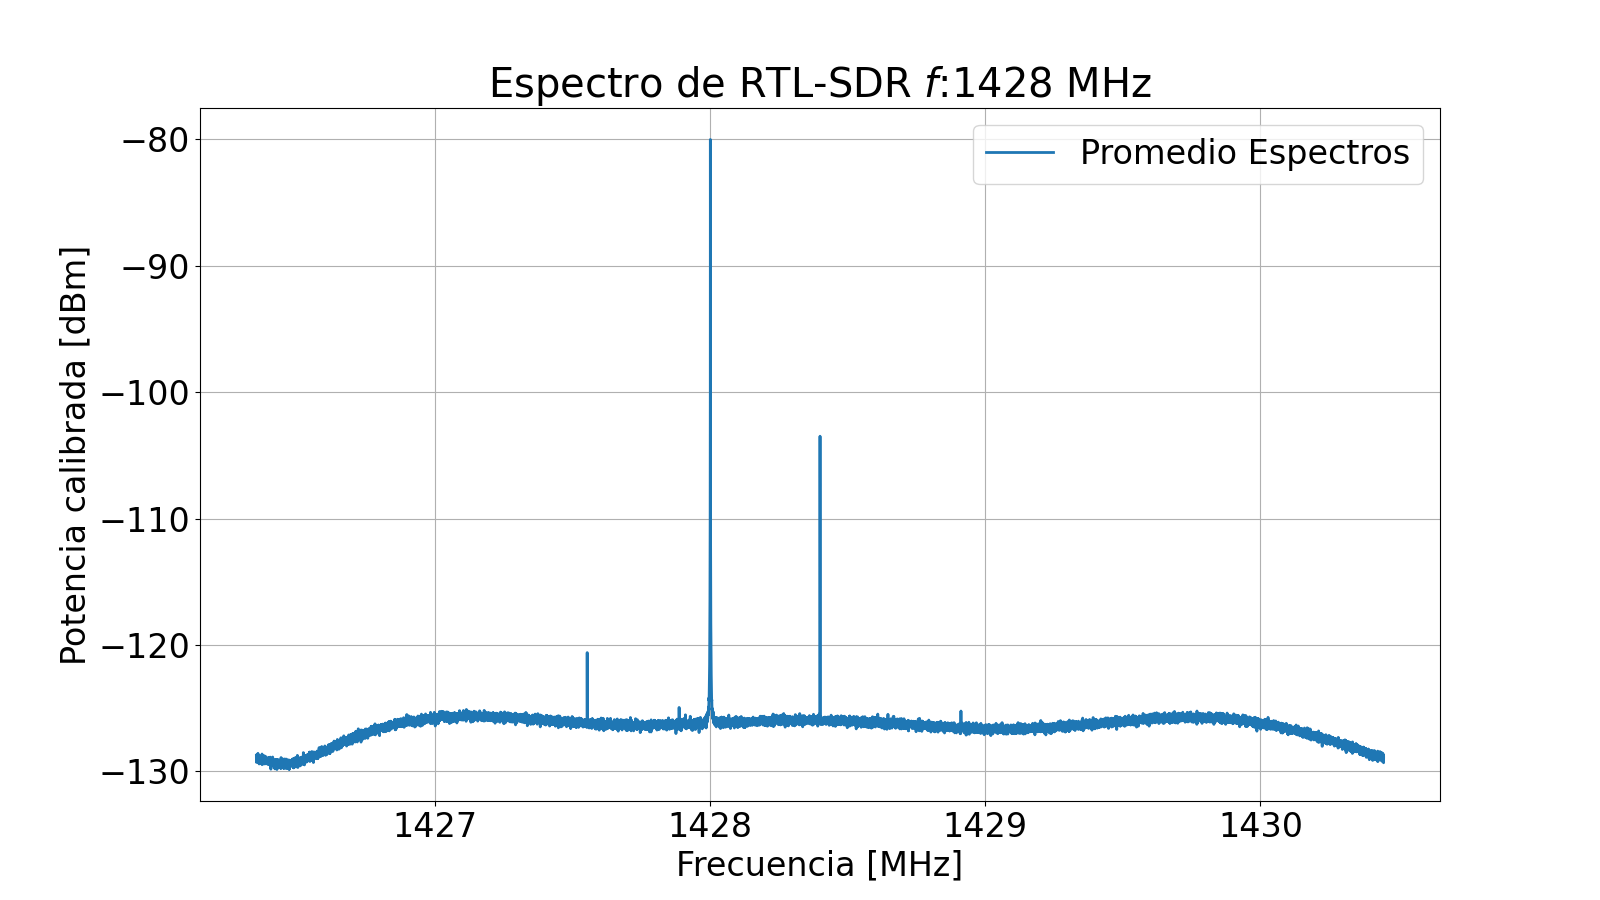
\includegraphics[width=0.8\textwidth]{img/rtl1428}
    \caption{Espectro obtenido por la RTL-SDR a 1428 GHz calibrado a potencia}
    \label{fig:rtl1428}
\end{figure}


\begin{images}{Tono de -80 dBm a las frecuencias de interés}
    \addimageanum{img/rtl300}{width=8cm}
    \addimageanum{img/rtl1000}{width=8cm}

    \imagesnewline

    \addimageanum{img/rtl400}{width=8cm}
    \addimageanum{img/rtl1500}{width=8cm}

    \imagesnewline

    \addimageanum{img/rtl500}{width=8cm}
    \addimageanum{img/rtl1700}{width=8cm}

\end{images}

\section{Ganancia y Directividad}

Al considerar una apertura de 3 metros de diametro, se calculó la directividad a partir de definición teórica para la banda de 1428 MHz.\\

\begin{equation}
    D = \frac{4\pi A}{\lambda^2} = 2033.7
\end{equation}

También se calculó la directividad a partir de los Hazes de media potencia obtenidos en la sección \ref{sec:patron}, utilizando la aproximación de apertura circular uniforme para un reflector parabólico.\\

\begin{equation}
    D = \frac{38,933}{HPBW_{E}\cdot HPBW_{H}} = 2057.7
\end{equation}

Lo que se condice con el valor teórico con un error aproximado de un 1\%.\\

Luego utilizando las mediciones de potencia en la banda de 1428 MHz, una vez calibradas con la escala obtenida con la RTL-SDR en la figura \ref{fig:rtl1428}, se obtuvo una ganancia del sistema a partir de la ecuación de Friis con la estrella artificial.\\

La potencia inyectada en la antena de 3 dBi de la copa de agua fue de 2.23 dBm, el cable de 20 metros de longitud y el cable de 2 metros tiene una atenuación de 20.4 dB y 2.2 dB respectivamente a la frecuencia de 1428 MHz, las pérdidas de espacio libre son de 81.01 dB y la potencia medida en el receptor fue -67.22 dBm.\\

\begin{equation}
    P_{rx}(dBm) = P_{tx}(dBm) + G_{tx}(dB) + G_{rx}(dB) - 20log{R}(km) - 20log{f}(MHz) - L_{\Omega}(dB)
\end{equation}

\begin{equation}
    G_{rx} = -67.22 -2.23 - 3 + 81.01 + 20.4 + 2.2 = 31.16 (dB)
\end{equation}

Con lo que se obtiene una ganancia de 31.16 dB para la banda de 1428 MHz. Por consecuensia se puede determinar la eficiencia de apertura considerando la directividad obtenida a partir del patrón de radiación de $D=2057.7$.\\

\begin{equation}
    \varepsilon_{A} = \frac{G}{D} = \frac{1304.1}{2057.7} = 0.634
\end{equation}

\begin{equation}
    \varepsilon_{A} = 0.634
\end{equation}

Este valor de eficiencia de apertura en comparación con la eficiencia de apertura declarada por el fabricante es un poco menor, siendo la del fabricante de 0.65 para el rango de frecuencias entre 1.2 a 4 GHz.\\

\section{Error de apuntamiento}

\section{Ancho de banda}

\section{Primera luz}

\begin{figure}
    \centering
    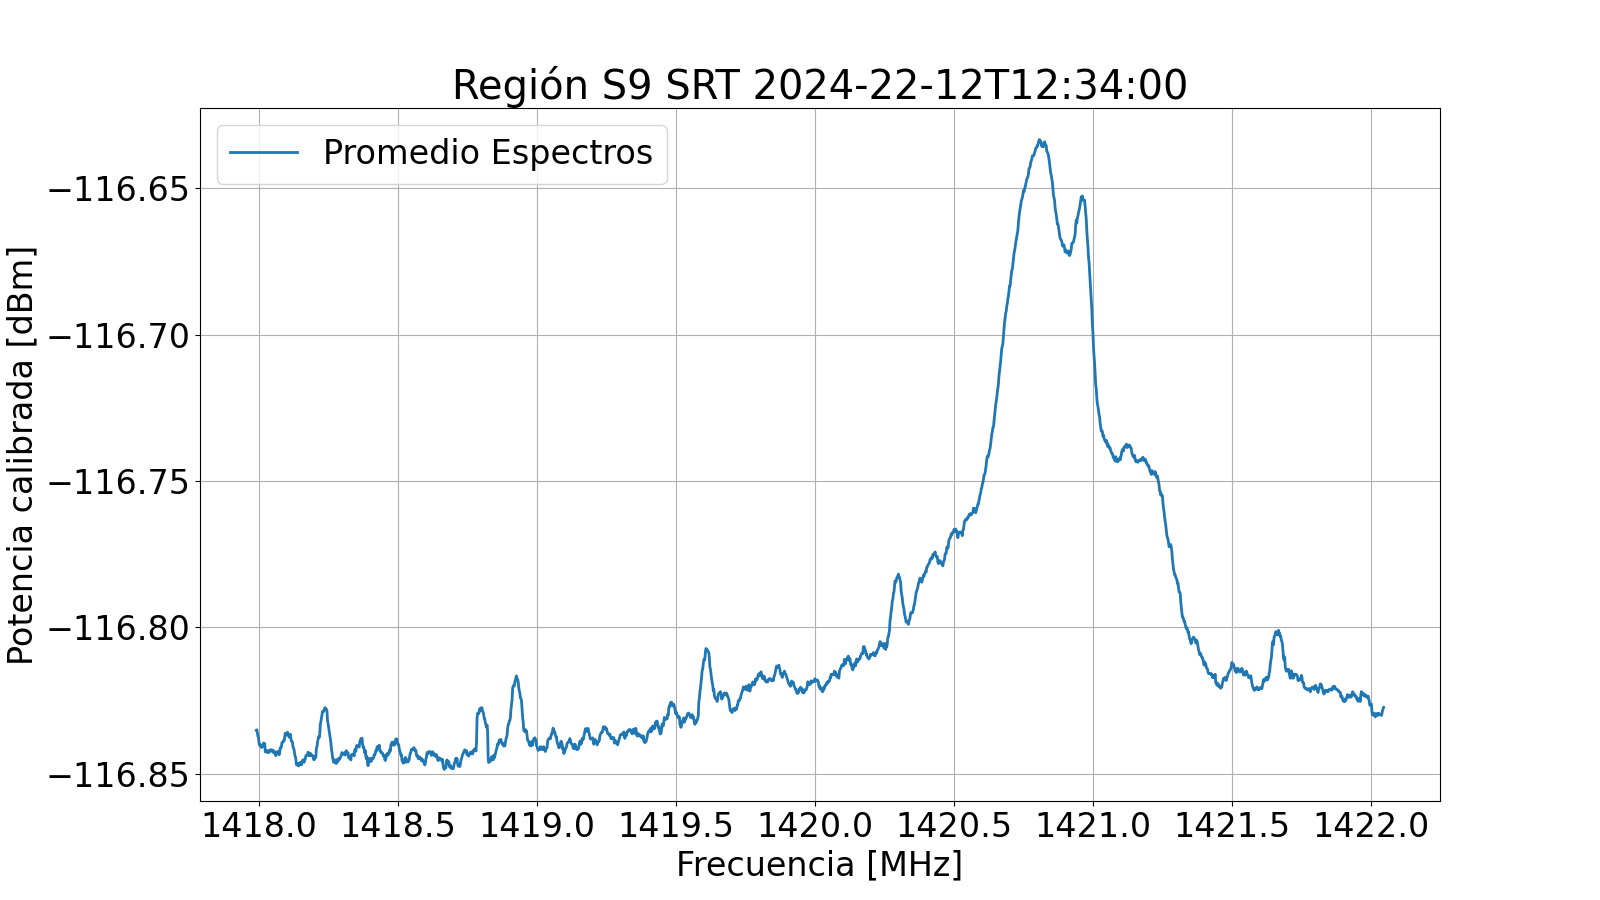
\includegraphics[width=0.8\textwidth]{img/h1}
    \caption{Espectro obtenido por la RTL-SDR a 1420 MHz calibrado a potencia}
    \label{fig:rtl1428}
\end{figure}